\documentclass[tikz,border=8pt]{standalone}
\usepackage[T1]{fontenc}
\usepackage{lmodern}
\usetikzlibrary{arrows.meta,positioning,calc}
\definecolor{ink}{HTML}{283746}
\definecolor{accent}{HTML}{285D85}
\begin{document}
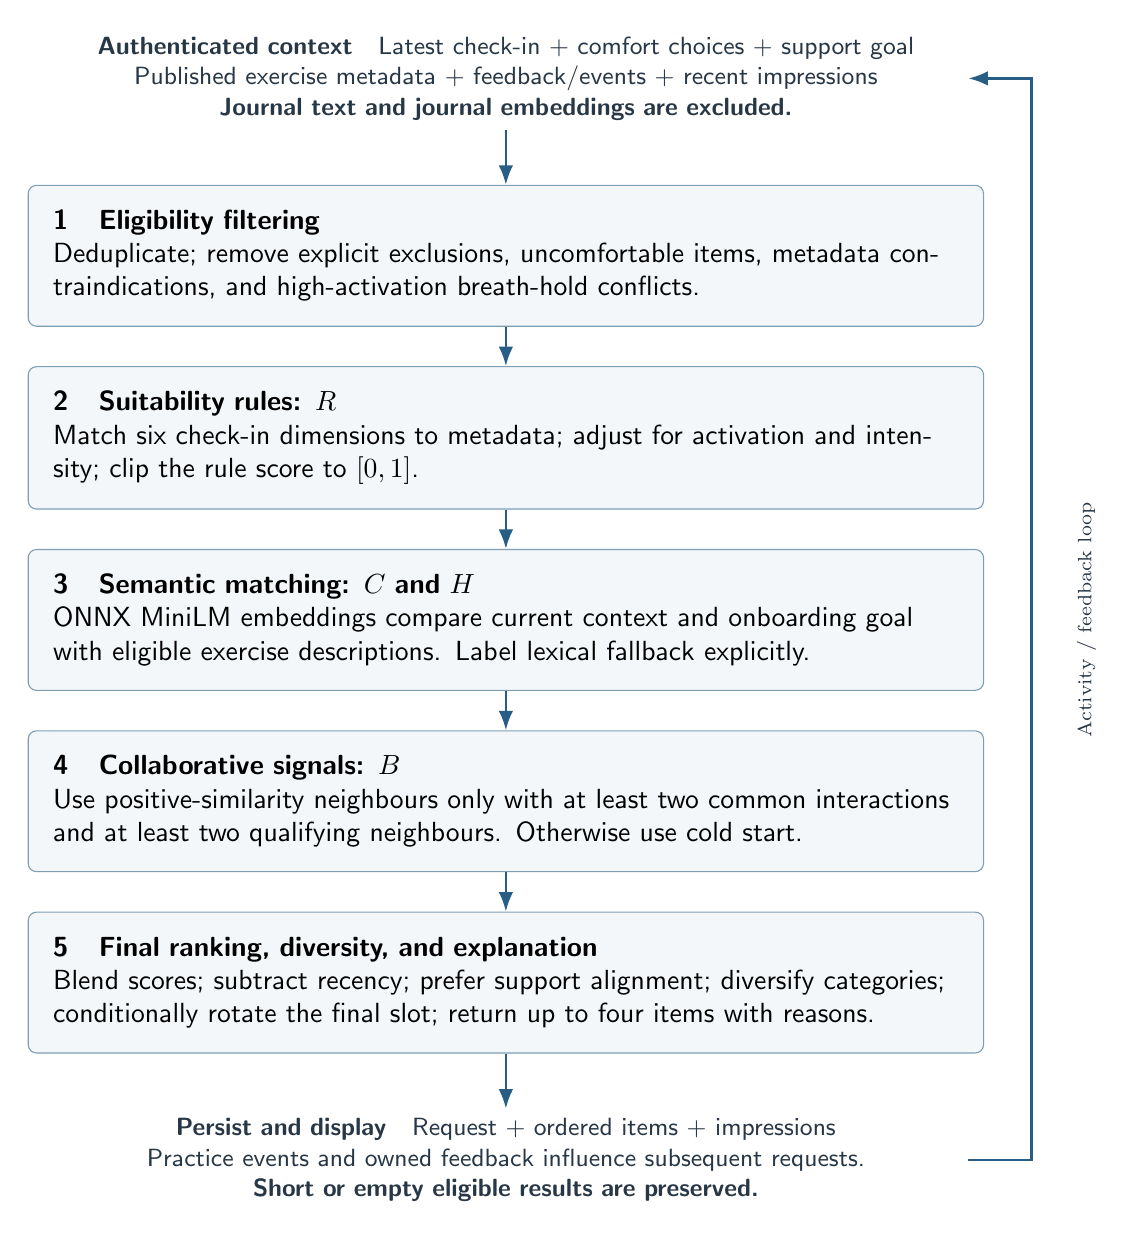
\begin{tikzpicture}[font=\sffamily,>=Latex,
 stage/.style={draw=accent!60,fill=accent!5,rounded corners=3pt,text width=11.5cm,align=left,inner sep=9pt},
 flow/.style={->,line width=0.9pt,draw=accent},
 note/.style={text width=11.5cm,align=center,font=\sffamily\small,text=ink}]
\node[note] (input) {\textbf{Authenticated context}\quad Latest check-in + comfort choices + support goal\\Published exercise metadata + feedback/events + recent impressions\\\textbf{Journal text and journal embeddings are excluded.}};
\node[stage,below=7mm of input] (one) {\textbf{1\quad Eligibility filtering}\\Deduplicate; remove explicit exclusions, uncomfortable items, metadata contraindications, and high-activation breath-hold conflicts.};
\node[stage,below=5mm of one] (two) {\textbf{2\quad Suitability rules: $R$}\\Match six check-in dimensions to metadata; adjust for activation and intensity; clip the rule score to $[0,1]$.};
\node[stage,below=5mm of two] (three) {\textbf{3\quad Semantic matching: $C$ and $H$}\\ONNX MiniLM embeddings compare current context and onboarding goal with eligible exercise descriptions. Label lexical fallback explicitly.};
\node[stage,below=5mm of three] (four) {\textbf{4\quad Collaborative signals: $B$}\\Use positive-similarity neighbours only with at least two common interactions and at least two qualifying neighbours. Otherwise use cold start.};
\node[stage,below=5mm of four] (five) {\textbf{5\quad Final ranking, diversity, and explanation}\\Blend scores; subtract recency; prefer support alignment; diversify categories; conditionally rotate the final slot; return up to four items with reasons.};
\node[note,below=7mm of five] (output) {\textbf{Persist and display}\quad Request + ordered items + impressions\\Practice events and owned feedback influence subsequent requests.\\\textbf{Short or empty eligible results are preserved.}};
\foreach \a/\b in {input/one,one/two,two/three,three/four,four/five,five/output} \draw[flow] (\a.south)--(\b.north);
\draw[flow] (output.east)--++(8mm,0)|-(input.east);
\node[rotate=90,font=\scriptsize,text=ink] at ($(three.east)+(13mm,0)$) {Activity / feedback loop};
\end{tikzpicture}
\end{document}
